% Slides for 2025-07-22
% To create a slide, use the following:
% \begin{frame}{TITLE}
%     BODY
% \end{frame}

% To create a slide with a bullet list, use the following:
% \begin{frame}{TITLE}
%     \begin{itemize}
%         \item ITEM 1
%         \item ITEM 2
%     \end{itemize}    
% \end{frame}

% To create a slide with numbered list, use the following:
% \begin{frame}{TITLE}
%     \begin{enumerate}
%         \item ITEM 1
%         \item ITEM 2
%     \end{enumerate}
% \end{frame}

% To create a slide with a graphic:
% 1. Add the graphic to this folder (named picture.png)
% 2. Use the following:
% \begin{frame}{TITLE}
%     \centering
%     \includegraphics[height=0.7\textheight,width=0.7\textwidth,keepaspectratio]{picture.png}
% \end{frame}

% To create a slide with two columns, use the following:
% \begin{frame}{TITLE}
%     \begin{columns}
%         \begin{column}{0.5\textwidth}
%             COLUMN 1 BODY
%         \end{column}
%         \begin{column}{0.5\textwidth}
%             COLUMN 2 BODY
%         \end{column}
%     \end{columns}
% \end{frame}

\begin{frame}{ML Team Agenda}
    \begin{itemize}
        \item EGCI work
        \item Spectrogram visualization
        \item Grad-CAM
        \item Williams et al. 2025
        \item Whale detection
        \item Template matching
        \item Next steps
    \end{itemize}
\end{frame}

\begin{frame}{EGCI Work}
    \begin{figure}
        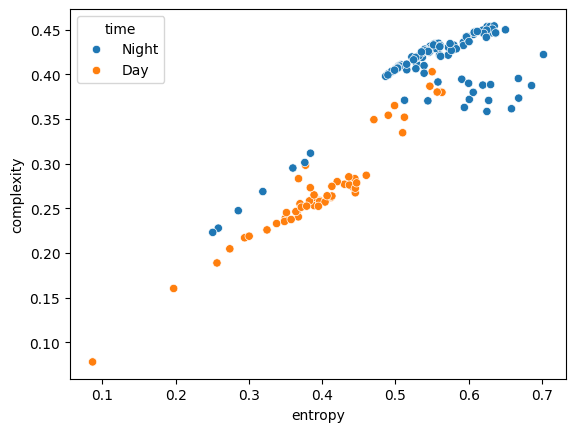
\includegraphics[height=0.7\textheight,width=0.7\textwidth,keepaspectratio]{images/muha_egci.png}
        \caption{Plot of EGCI against entropy for Muha's data, labeled with time of day}
    \end{figure}
\end{frame}

\begin{frame}{Spectrogram Visualization}
    High-dimensional spatial representation of audio clips
    \begin{figure}
        \centering
        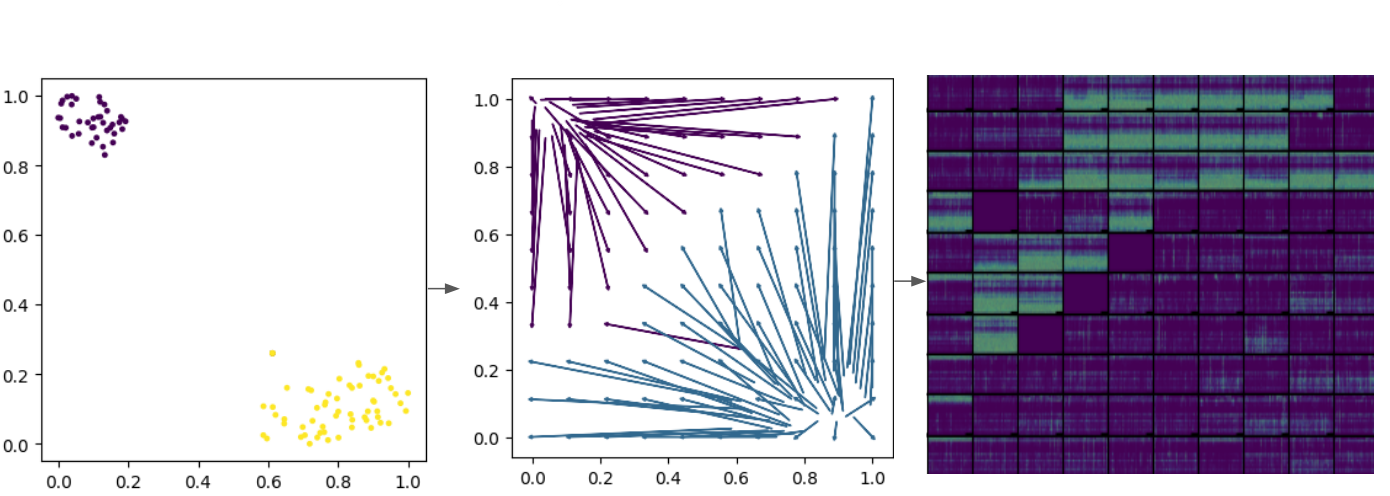
\includegraphics[height=0.85\textheight,width=0.85\textwidth,keepaspectratio]{images/spectrogram_visualization.png}
        \caption{Spectrogram visualization process of audio clips}
    \end{figure}
\end{frame}

\begin{frame}{Grad-CAM}
    \begin{columns}
        \begin{column}{0.5\textwidth}
            Degraded Grad-CAM:
            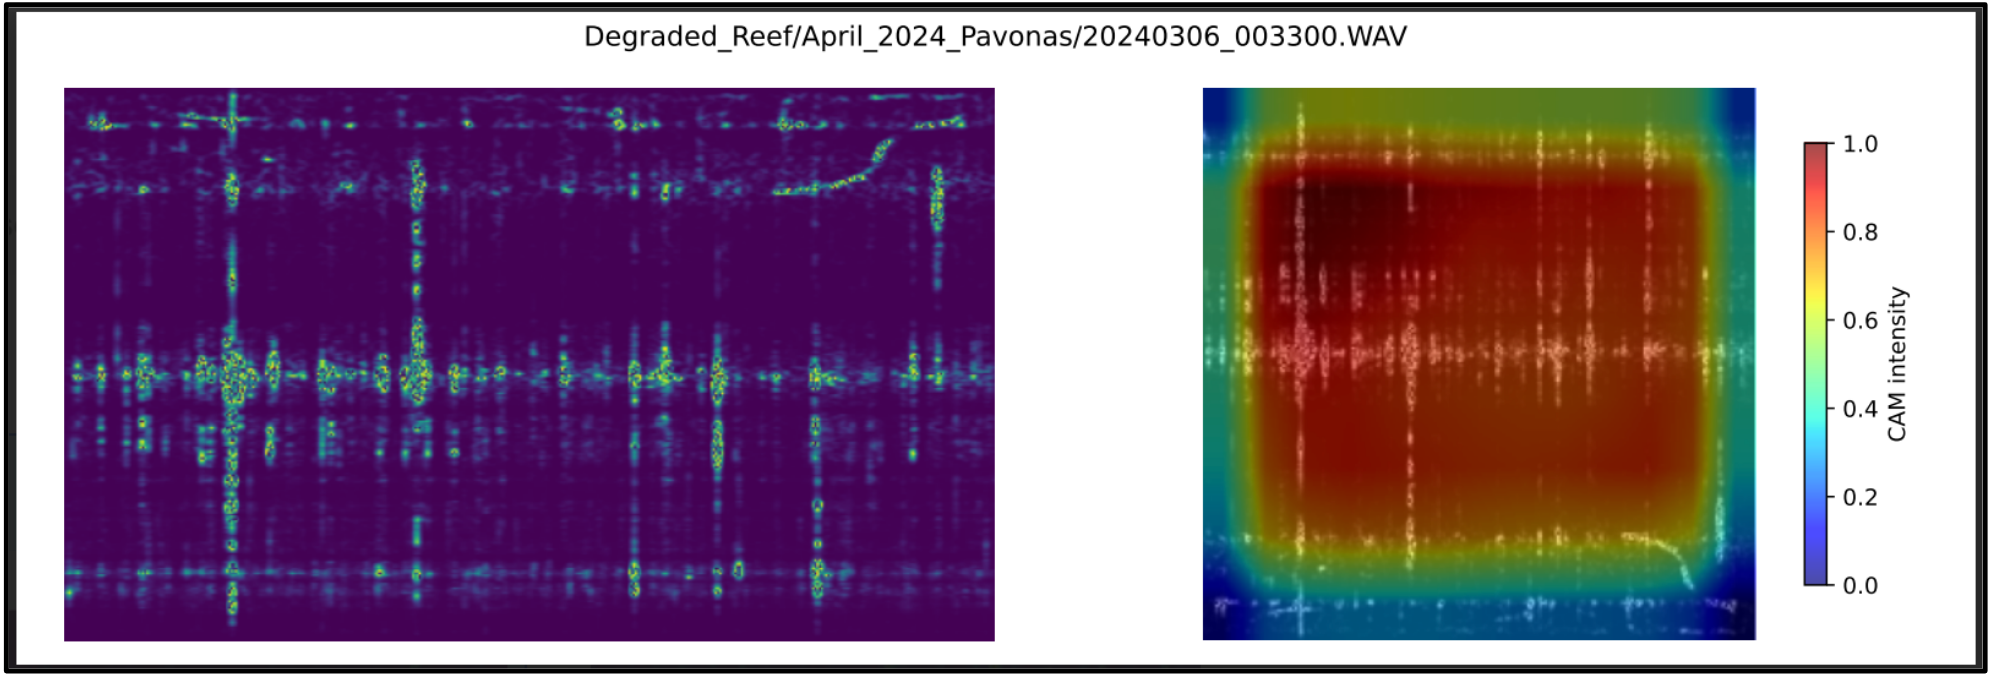
\includegraphics[height=1.0\textheight,width=1.0\textwidth,keepaspectratio]{images/degraded_grad_cam.png}
        \end{column}
        \begin{column}{0.5\textwidth}
            Non-degraded Grad-CAM:
            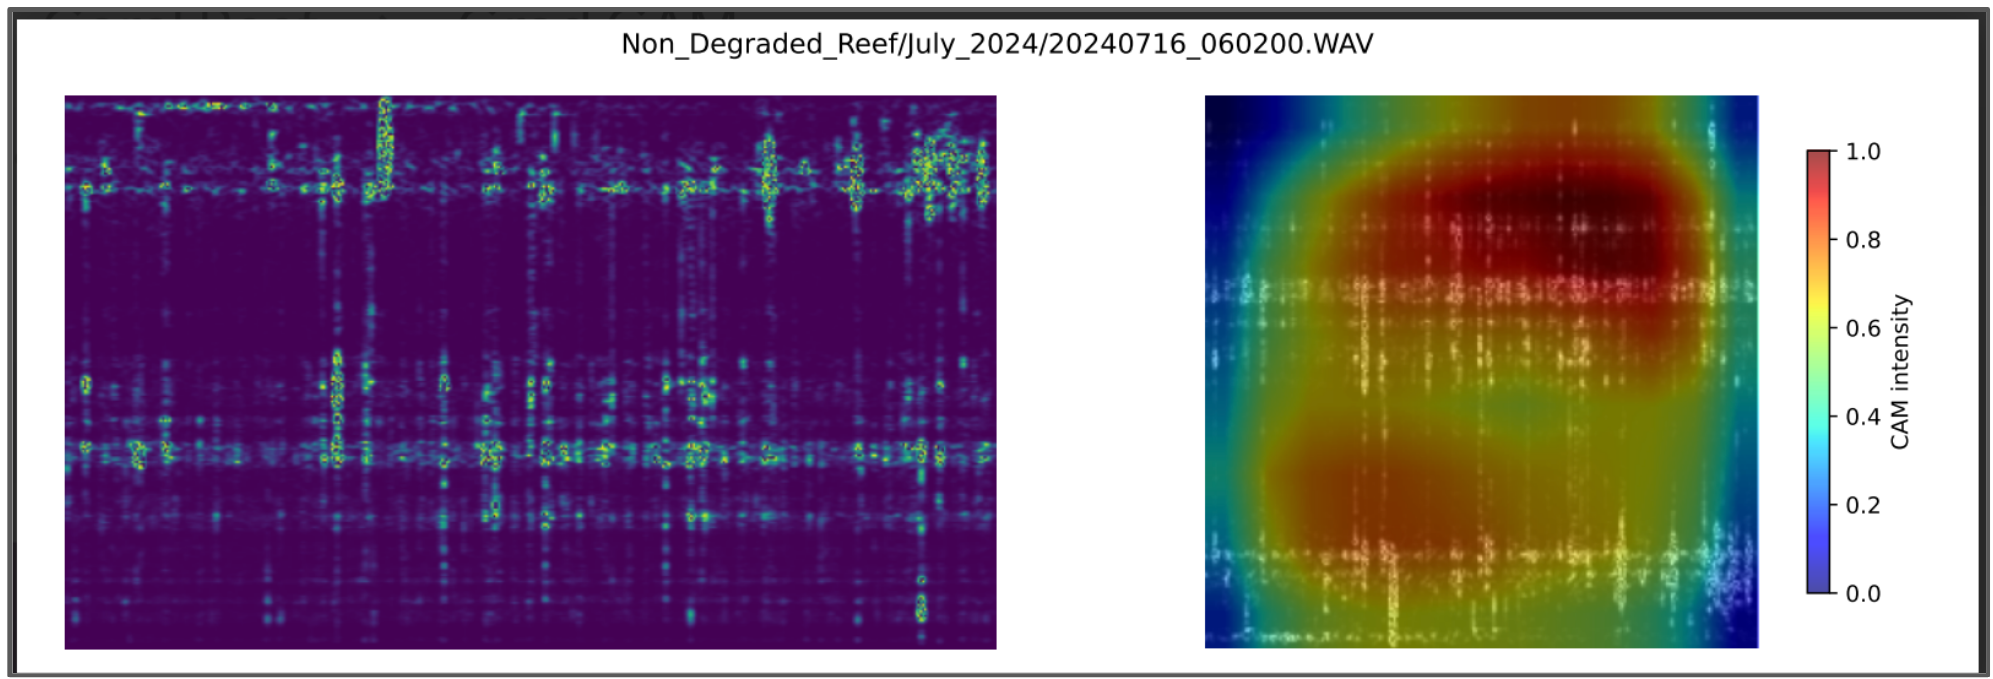
\includegraphics[height=1.0\textheight,width=1.0\textwidth,keepaspectratio]{images/non_degraded_grad_cam.png}
        \end{column}
    \end{columns}
\end{frame}

\begin{frame}{Grad-CAM Results}
    Sample of 200 degraded and non-degraded audio clips
    \begin{figure}
        \centering
        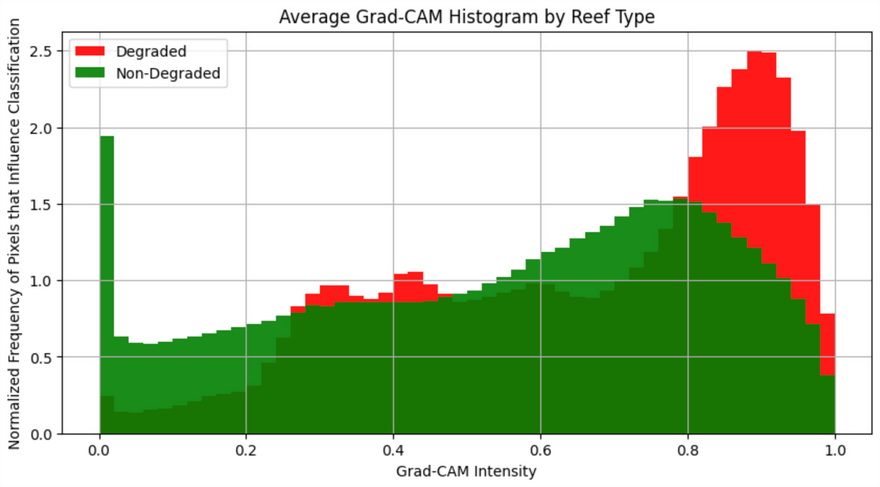
\includegraphics[height=0.6\textheight,width=0.6\textwidth,keepaspectratio]{images/grad_cam_histogram.png}
        \caption{Grad-CAM histogram}
    \end{figure}
\end{frame}

\begin{frame}{Williams et al. 2025}
    \begin{itemize}
        \item Using SurfPerch on Paola's data
    \end{itemize}
    % Williams et al. 2025: https://royalsocietypublishing.org/doi/10.1098/rstb.2024.0280
    % SurfPerch: https://www.kaggle.com/models/google/surfperch
\end{frame}

\begin{frame}{Whale Detection}
    \begin{itemize}
        \item Can use multispecies-whale model to detect data containing whale vocalizations
        \item These clips can then be filtered out
    \end{itemize}
    % multispecies-whale model: https://www.kaggle.com/models/google/multispecies-whale
\end{frame}

\begin{frame}{Template Matching}
    \begin{itemize}
        \item Can take a reference sound and compare it with the data to find recordings containing said sound
        \item Implementing this with Muha's liked sounds
    \end{itemize}
\end{frame}

\begin{frame}{Next Steps}
    \begin{itemize}
        \item Create interactive website for Muha
        \item Work on knowledge graphs
        \item Continue with template matching work
    \end{itemize}
\end{frame}

\begin{frame}{Collar Team Agenda}
    \begin{itemize}
        \item 
    \end{itemize}
\end{frame}